\documentclass[aspectratio=169]{beamer}

% Je kan het lettertype iets vergroten door hierboven optie ``14pt'' toe te
% voegen.

%==============================================================================
% Aanloop
%==============================================================================

%---------- Vormgeving --------------------------------------------------------

\usetheme{hogent}

% Kies hieronder een achtergrondkleur
\usecolortheme{hgwhite} % witte achtergrond, zwarte tekst
%\usecolortheme{hgblack} % zwarte achtergrond, witte tekst

%---------- Packages ----------------------------------------------------------

\usepackage[dutch]{babel}      % Nederlandse taal: splitsingen, enz.

\usepackage{booktabs}          % Mooie tabellen
\usepackage{multirow,multicol} % Tabelcellen samenvoegen
\usepackage{eurosym}           % Euro symbool
\usepackage{hyperref}
\hypersetup{
    colorlinks=true,
    linkcolor=blue,
    filecolor=magenta,      
    urlcolor=cyan,
    pdftitle={Overleaf Example},
    pdfpagemode=FullScreen,
}

\urlstyle{same}

%---------- Commando-definities -----------------------------------------------

%---------- Info over de presentatie ------------------------------------------

\title[Korte titel]{Google Scholar zoekresultaten voor wetenschappelijke projecten: linked data \& natural language processing}
\author{Bart De Paepe}
\date{\today}

%==============================================================================
% Inhoud presentatie
%==============================================================================

\begin{document}

%---------- Titelpagina, inhoudstafel -----------------------------------------

\frame{\maketitle}

\begin{frame}
  \frametitle{Inhoud.}

  \tableofcontents
\end{frame}
 
%---------- Corpus ------------------------------------------------------------

\section{Kader.}

\begin{frame}
  \frametitle{Vlaams Instituut voor de Zee}
  \begin{figure}
      \caption{website url: \url{https://www.vliz.be}}
      
      
\includegraphics[height=.4\textheight]
      {kader/VLIZ_LOGO.png}
      % Bron: https://www.pexels.com/photo/hand-on-cup-of-coffee-984536/
      \label{img:voorbeeld}
  \end{figure}
  
\end{frame}

\begin{frame}
    \frametitle{Integrated Marine Information System}
    \href{https://www.vliz.be/nl/imis}{Raadpleeg IMIS}
    
    
\end{frame}

\begin{frame}
    \frametitle{Google Scholar}
    \begin{columns}[c]
        % create the column with the first image, that occupies
        % half of the slide
        \begin{column}{.5\textwidth}
    \begin{figure}
        \caption{zoekopdracht}
        
        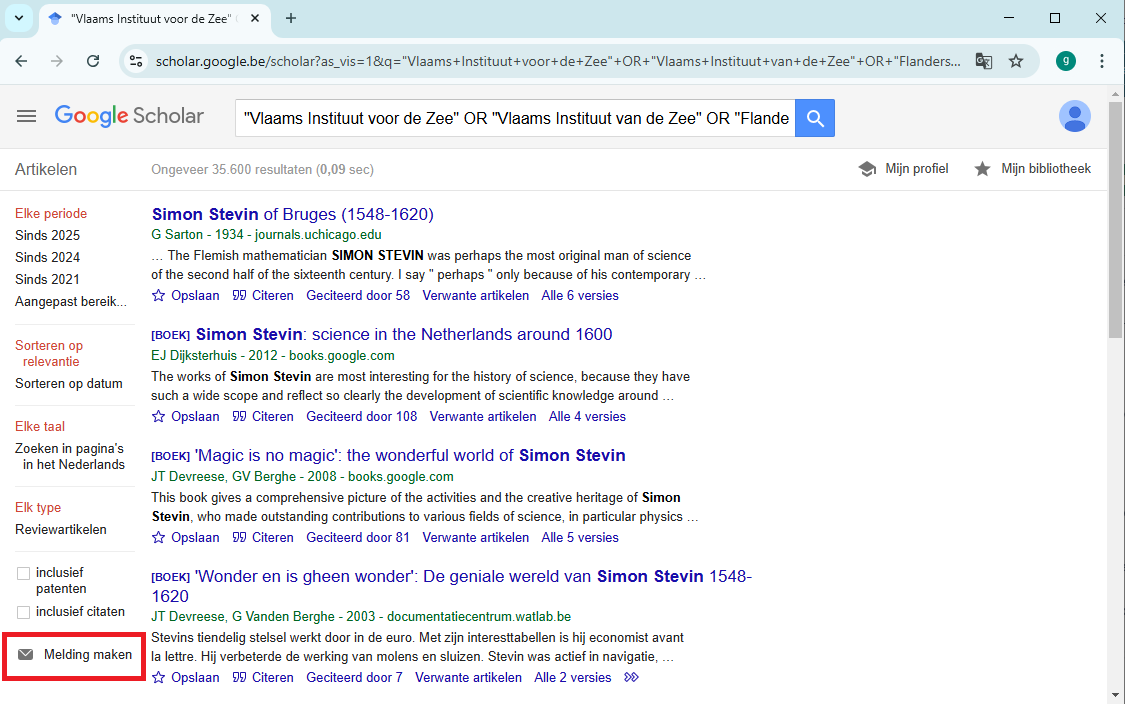
\includegraphics[height=.5\textheight]
        {kader/google-scholar/2_zoekresultaten.PNG}
        % Bron: https://www.pexels.com/photo/hand-on-cup-of-coffee-984536/
        \label{img:voorbeeld}
    \end{figure}
    \end{column}
    \begin{column}{.5\textwidth}
    \begin{figure}
        \caption{alert}
        
        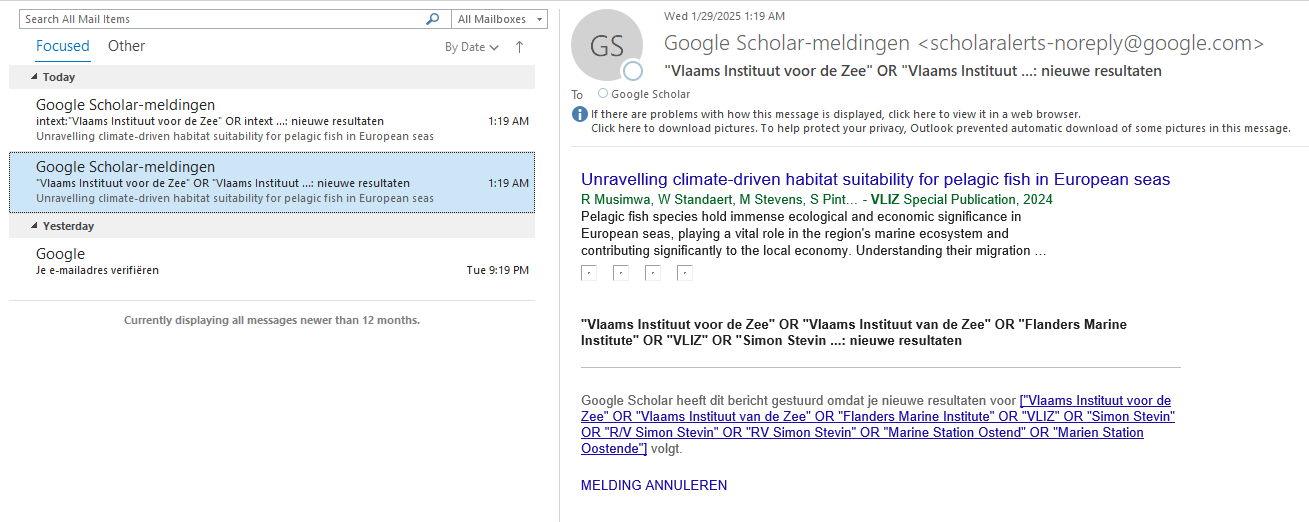
\includegraphics[height=.5\textheight]
        {kader/google-scholar/5_email.PNG}
        % Bron: https://www.pexels.com/photo/hand-on-cup-of-coffee-984536/
        \label{img:voorbeeld}
    \end{figure}
\end{column}
\end{columns}
    
    
\end{frame}

{
    \setbeamertemplate{background}[imgletter]%
    {kader/amin-zabardast-Q57aftqNKiE-unsplash.jpg}{P}
\begin{frame}
    \frametitle{Het probleem.}
    Photo by Amin Zabardast on https://unsplash.com/photos/a-street-sign-on-a-pole-next-to-a-building-Q57aftqNKiE
    
    
\end{frame}
}

\begin{frame}
    \frametitle{De onderzoeksvraag.}
    ``Hoe kunnen de zoekresultaten van Google Scholar automatisch toegevoegd worden aan IMIS?''
    \begin{itemize}
        \item Hoe kunnen de uiteenlopende zoekresultaten van Google Scholar omgezet worden in gestructureerde data?
        \item Zijn alle zoekresultaten uniek identificeerbaar zodat er geen duplicaten opgeslagen worden?
    \end{itemize}
    \begin{itemize}
        \item Hoe kunnen ook steeds nieuwe zoekresultaten van dezelfde zoekopdracht systematisch opgezocht worden?
        \item Kan er een score berekend worden hoe relevant elk zoekresultaat is ten opzichte van de zoekopdracht?
        \item Als er geen unieke identifier is, hoe wordt er dan gecontroleerd op duplicaten? 
    \end{itemize}
    \begin{itemize}
        \item Hoe blijft de tool overwegend onafhankelijk van third-party software?
        \item Hoe wordt er gegarandeerd dat de tool op de bestaande hardware kan draaien? 
    \end{itemize}
    
    
\end{frame}

\begin{frame}
    \frametitle{Proof of Concept bouwen.}
    Geen grappige afbeelding met auteursrechten hier, wel \href{https://www.slideserve.com/zocha/agile-project-management}{daar}.
    
    
    
\end{frame}

{
    \setbeamertemplate{background}[pure]{methode/arrow.png}
\section{Methode.}
}

\begin{frame}
    \frametitle{Web scraping.}
    
    
\end{frame}

\begin{frame}
\frametitle{Natural language processing.}


\end{frame}

\begin{frame}
\frametitle{Linked data.}


\end{frame}

\begin{frame}
\frametitle{Semantic search.}


\end{frame}

\section{Resultaten.}

\begin{frame}
\frametitle{Resultaten.}


\end{frame}

\section{Discussie.}

\begin{frame}
\frametitle{Discussie.}


\end{frame}

\section{Conclusie.}

\begin{frame}
\frametitle{Conclusie.}


\end{frame}

\end{document}
